\documentclass[
size=17pt,
paper=smartboard,
mode=present,
display=slidesnotes,
style=paintings,
nopagebreaks,
blackslide,
fleqn]{powerdot}

% styles: sailor, paintings
% wj capsules prettybox
% mode = handout or present


\usepackage{amsmath,graphicx,color,amsfonts}
\usepackage[brazilian]{babel}
\usepackage[utf8]{inputenc}
\newcommand{\palette}{Europa}


% palettes:
%    - sailor: Sea, River, Wine, Chocolate, Cocktail 
%    - paintings: Syndics, Skater, GoldenGate, Moitessier, PearlEarring, Lamentation, HolyWood, Europa, MayThird, Charon 

\newcommand{\cursopequeno}{EC01008 AOC}
\newcommand{\cursogrande}{\Large EC01008 -- Arquitetura e organização de computadores}



\author{Ronaldo de Freitas Zampolo\\FCT-ITEC-UFPA}
\date{2023-4}


\pdsetup{
   lf = {\cursopequeno},
   rf = {Desempenho}, palette = {\palette}, randomdots={false},
   cf = {\theslide}
}


%opening
\title{\cursogrande\\ \vspace{1cm}Desempenho de computadores}

\begin{document}
   \maketitle[randomdots={false}]
   
   \begin{slide}{Agenda}
      \tableofcontents[content=sections]
   \end{slide}
%%%%%%%%%%%%%%%%%%%%%%%%%%%%%%%%%%%%%%%%%%%%%%%%%%%%%%
\section[slide=true]{Projeto visando ao desempenho}
\begin{slide}[toc=]{Demanda por maior velocidade}
	\begin{itemize}
		\item Aplicações mais sofisticadas vs. sistemas computacionais de maior desempenho: realimentação mútua\pause 
		\item Exemplos de aplicações que exigem grande poder de processamento:
			\begin{itemize}
				\item Processamento de imagem/vídeo
				\item Gráficos 3D
				\item Reconhecimento de voz
				\item Videoconferência\pause
			\end{itemize}
		\item Elementos a considerar:
			\begin{itemize}
				\item Microprocessador: não está sozinho no sistema\pause
				\item Memória: sua interface com o processador é de especial importância para execução eficiente de instruções\pause
				\item Dispositivos periféricos: muita diversidade aqui em termos de velocidade\pause
				\item Estrutura de interconexão: hierarquia de barramentos para lidar com a diversidade de maneira eficiente
			\end{itemize}
	\end{itemize}
\end{slide}


\begin{slide}[toc=]{Microprocessadores}
	\begin{itemize}
		\item Maior integração com o passar do tempo (Lei de Moore):\pause
			\begin{itemize}
				\item Redução do tamanho das portas lógicas
				\item Portas lógicas mais próximas
				\item Redução no tempo de propagação dos sinais
				\item Maior \textit{clock}
				\item Estreitamento das trilhas de condução\pause
				\item Problemas:
					\begin{itemize}
						\item Aumento de potência dissipada (aumento de custo, e aquecimento)\pause
						\item Trilhas mais estreitas, aumentam a resistência (R)\pause
						\item Trilhas mais próximas aumentam o efeito de acoplamento capacitivo (C)     \pause
						\item Aumento do atraso à medida que o produto RC aumenta
					\end{itemize}
			\end{itemize}
	\end{itemize}
\end{slide}

\begin{slide}[toc=]{Micropocessadores}
	\begin{itemize}
		\item Estratégias para manter o processador ocupado:\pause
			\begin{itemize}
				\item Pipeline: 
					\begin{itemize}
      						\item Permite execução de instruções em paralelo
						\item Funciona como uma linha de montagem
						\item Diferentes estágios de execução de diferentes instruções ao mesmo tempo:\pause
							\begin{itemize}
								\item Busca (envolve Memória e Barramentos)
								\item Decodificação (envolve Unidade de Controle)
								\item Execução (envolve ULA)\pause
							\end{itemize}
					\end{itemize}
				\item Predição de desvio: busca antecipada de instruções prováveis \pause
				\item Execução superescalar: execução de múltiplos \textit{pipelines} em paralelo\pause
				\item Análise de fluxo de dados: 
					\begin{itemize}
						\item Avaliação de dependência de dados entre instruções
						\item Não havendo dependência, executar\pause
					\end{itemize}
				\item Execução especulativa: predição de desvio + análise de fluxo de dados
			\end{itemize}
	\end{itemize}
\end{slide}


\begin{slide}[toc=]{Comparativo de velocidade}
	\begin{center}
		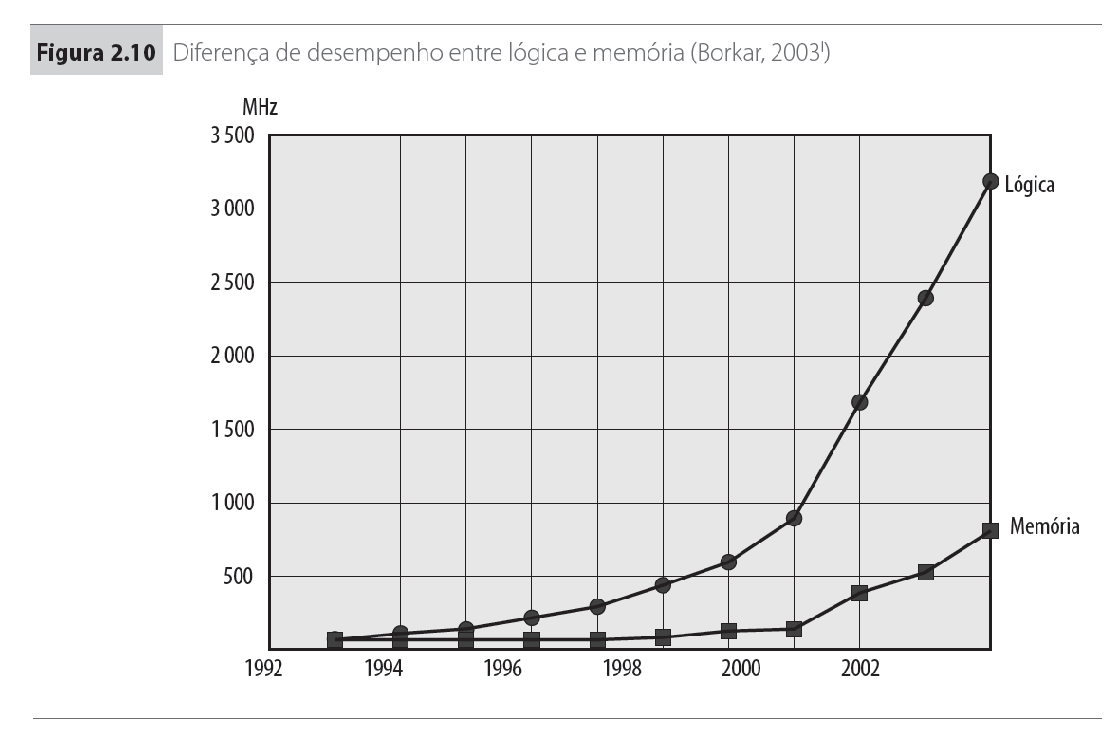
\includegraphics[width=0.80\textwidth]{figs/diff_proc_mem.eps} 
	\end{center}
\end{slide}
\begin{slide}[toc=]{Memória}
	\begin{itemize}
		\item A velocidade de transferência de dados entre memória e processador é um fator crítico no desempenho\pause
		\item Possibilidades:
			\begin{itemize}
				\item Aumentar número de bits recuperados de uma só vez: DRAM ``mais larga'' ao invés de ``mais profunda''\pause
				\item Mudar interface da DRAM: inclusão de memória cache ou outros técnicas semelhantes \pause
				\item Reduzir frequência de acesso à memória: cache de vários níveis e caches on-chip\pause
				\item Aumentar largura de banda de interconexão:
					\begin{itemize}
						\item Barramentos de alta velocidade
						\item Hierarquia de barramentos\pause
					\end{itemize}
			\end{itemize}
		\item Atualmente, aproximadamente metade da área de um chip processador é ocupado com memória cache
	\end{itemize}
\end{slide}

\begin{slide}[toc=]{Dispositivos periféricos}
	Taxa de dados de alguns periféricos
	\begin{center}
		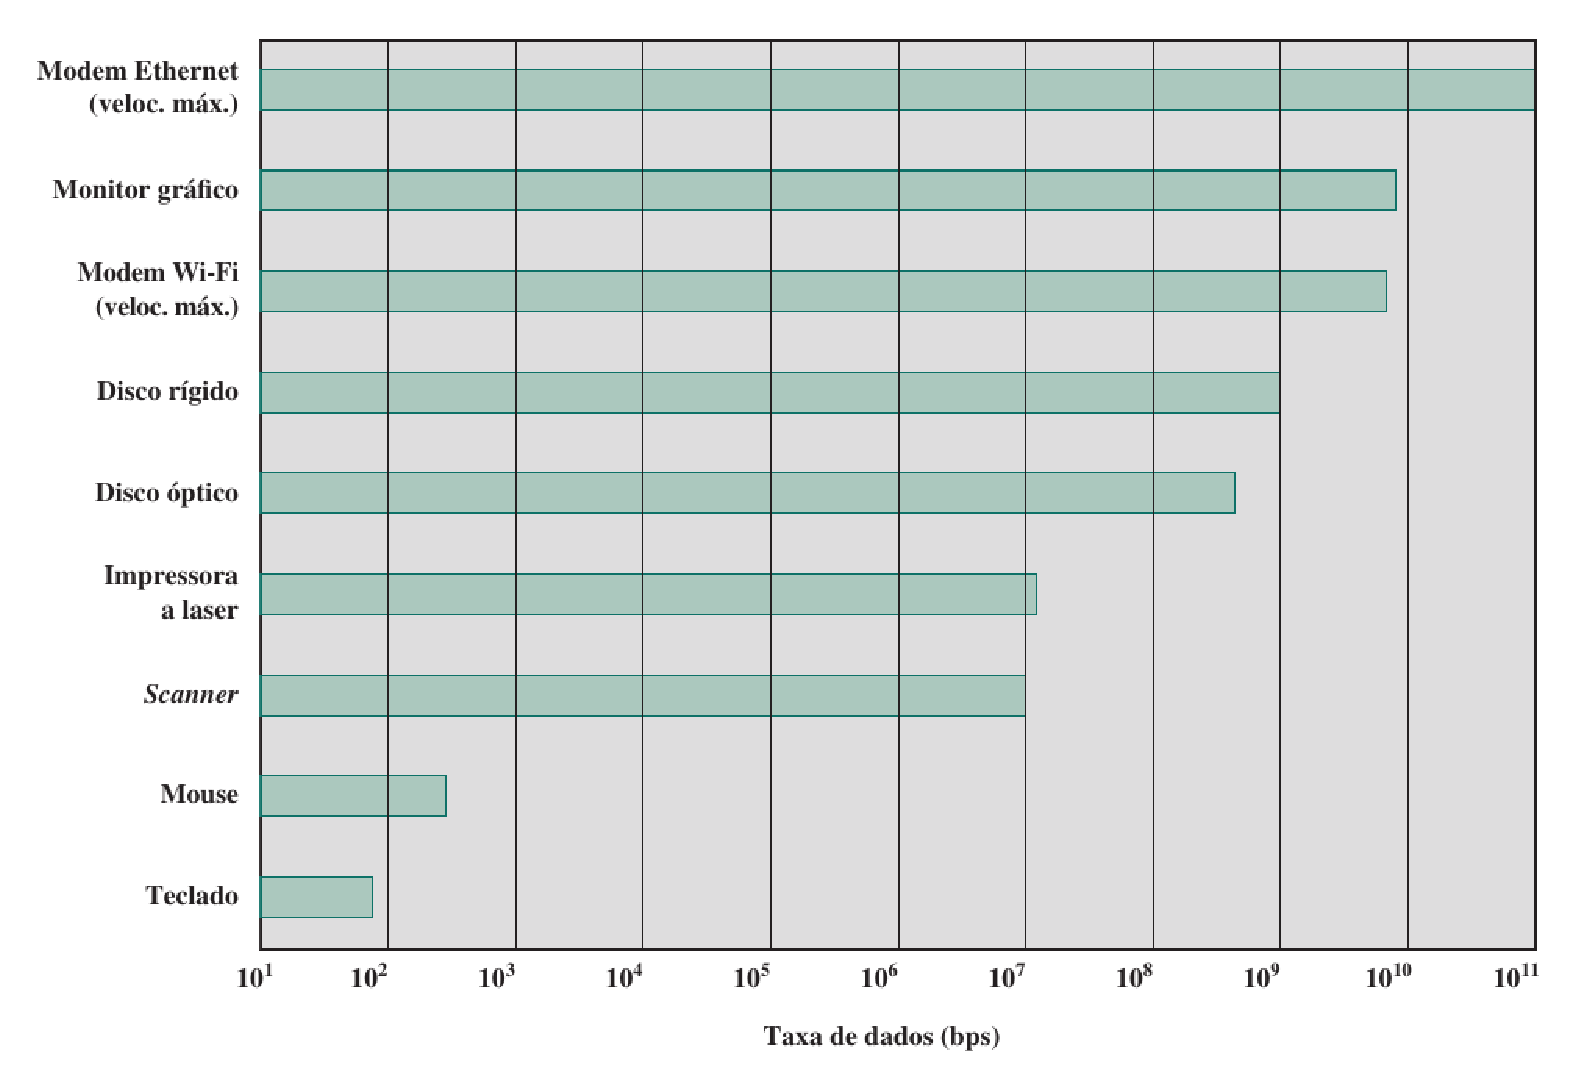
\includegraphics[width=0.7\textwidth]{figs/taxa-dados}
	\end{center}
\end{slide}

\section[slide=true]{Multicore, MIC e GPGPU}
\begin{slide}[toc=]{Novas tendências de projeto}
	\begin{itemize}
		\item O desempenho em um processador é proporcional à raiz quadrada da complexidade\pause
		\item Dobrar o número de processadores, dobra o desempenho (software precisa estar adaptado ao processamento por dois processadores)\pause
		\item É mais vantajoso: trocar um processador mais complexo por dois mais simples\pause
		\item Tendência: Multicore 
			\begin{itemize}
				\item Vários processadores iguais (sistema homogêneo) em um único chip\pause
				\item Memória cache on chip (com capacidade cada vez maior) compartilhada\pause
				\item Quantidade de processadores (núcleos): 2, 4, 8, 16, 32, ..., 50 !! (many integrated core -- MIC)\pause
			\end{itemize}
		\item Tendência: uso de GPUs
			\begin{itemize}
				\item GPU (graphics processing unit): processadores de propósito específico para tratamento de imagem e vídeo\pause
				\item Multicore + GPU: general-purpose computing on GPU (GPGPU)
			\end{itemize}
	\end{itemize}
\end{slide}

\begin{slide}[toc=]{Micropocessadores}
	Tendência atual no desenvolvimento de processadores
	\begin{center}
		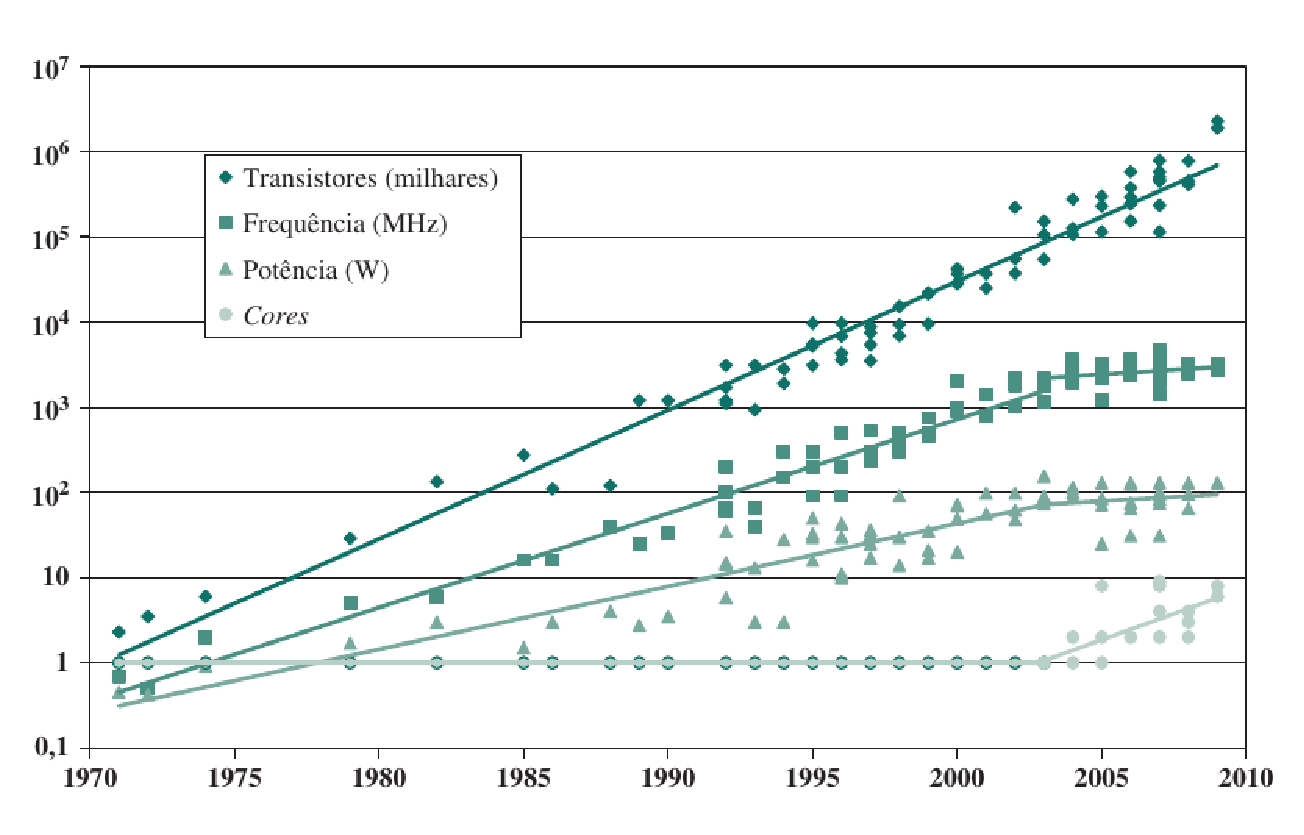
\includegraphics[width = 0.8\textwidth]{figs/tendencia}
	\end{center}
\end{slide}

\section[slide=true]{Leis de Amdahl e Little}
\begin{slide}{Lei de Amdahl (Gene Amdahl, 1967)}
\begin{itemize}
   \item Caracteriza o \textit{speedup} de um programa usando múltiplos processadores em comparação com um único processador:
   \begin{align*}
      \text{Speedup} &= \frac{\text{tempo de execução com um único processador}}{\text{tempo de execução com $N$ processadores paralelos}}\\
              &= \frac{T(1-f)+Tf}{T(1-f)+\frac{Tf}{N}}\\
              &= \frac{1}{(1-f)+\frac{f}{N}}\\
   \end{align*}
   onde $f$ corresponde à fração paralelizável.\pause
		\item Consequências:
			\begin{itemize}
				\item Quando $f$ é pequeno, o uso de processadores em paralelo tem pouco efeito
				\item Quando $N$ tende ao infinito, o \emph{speedup} atinge um limite
			\end{itemize}
\end{itemize}
\end{slide}

\begin{slide}{Lei de Amdahl }
	\begin{itemize}
		\item Ilustração da Lei de Amdahl
			\begin{center}
				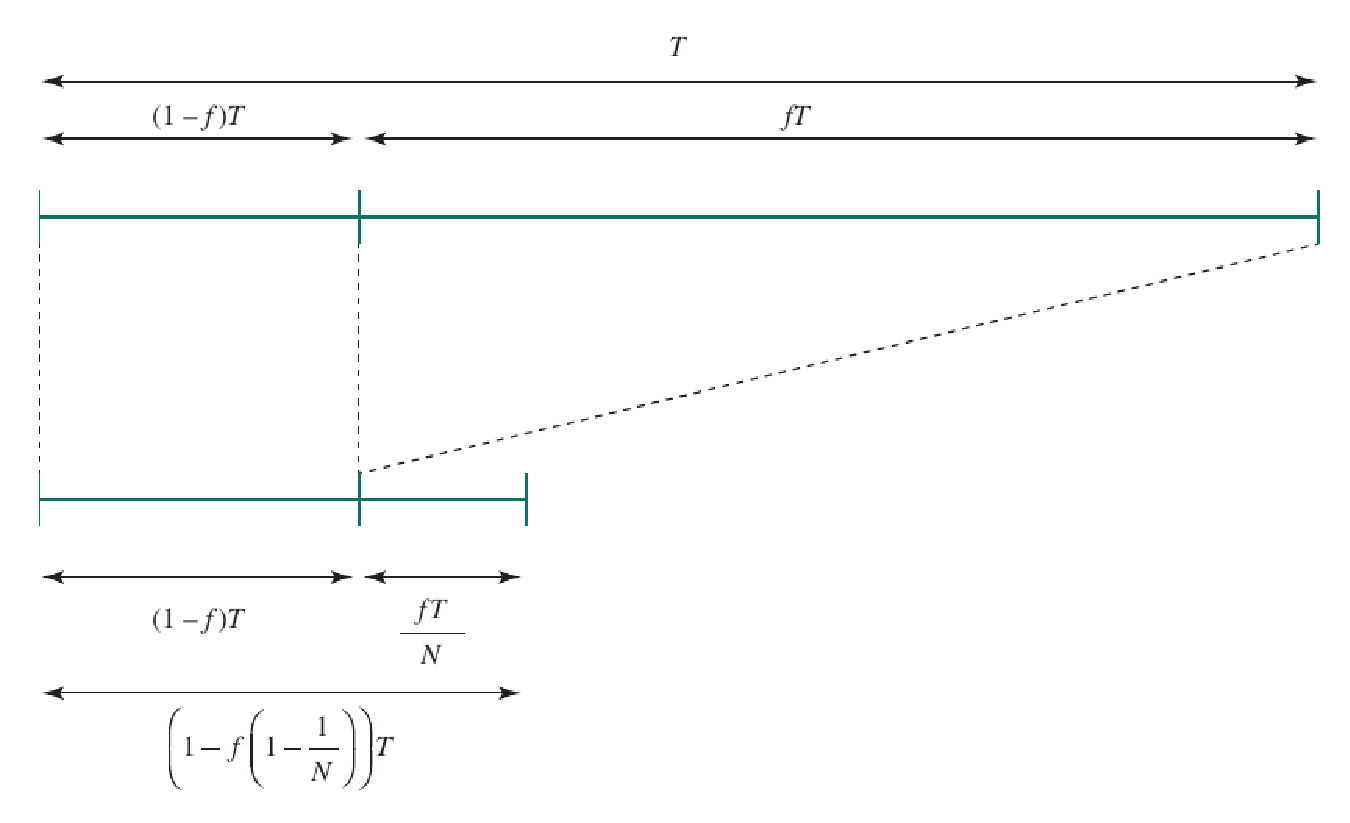
\includegraphics[width=0.8\textwidth]{figs/amdahl1}
			\end{center}
	\end{itemize}
\end{slide}

\begin{slide}{Lei de Amdahl }
	\begin{itemize}
		\item Ilustração da Lei de Amdahl
			\begin{center}
				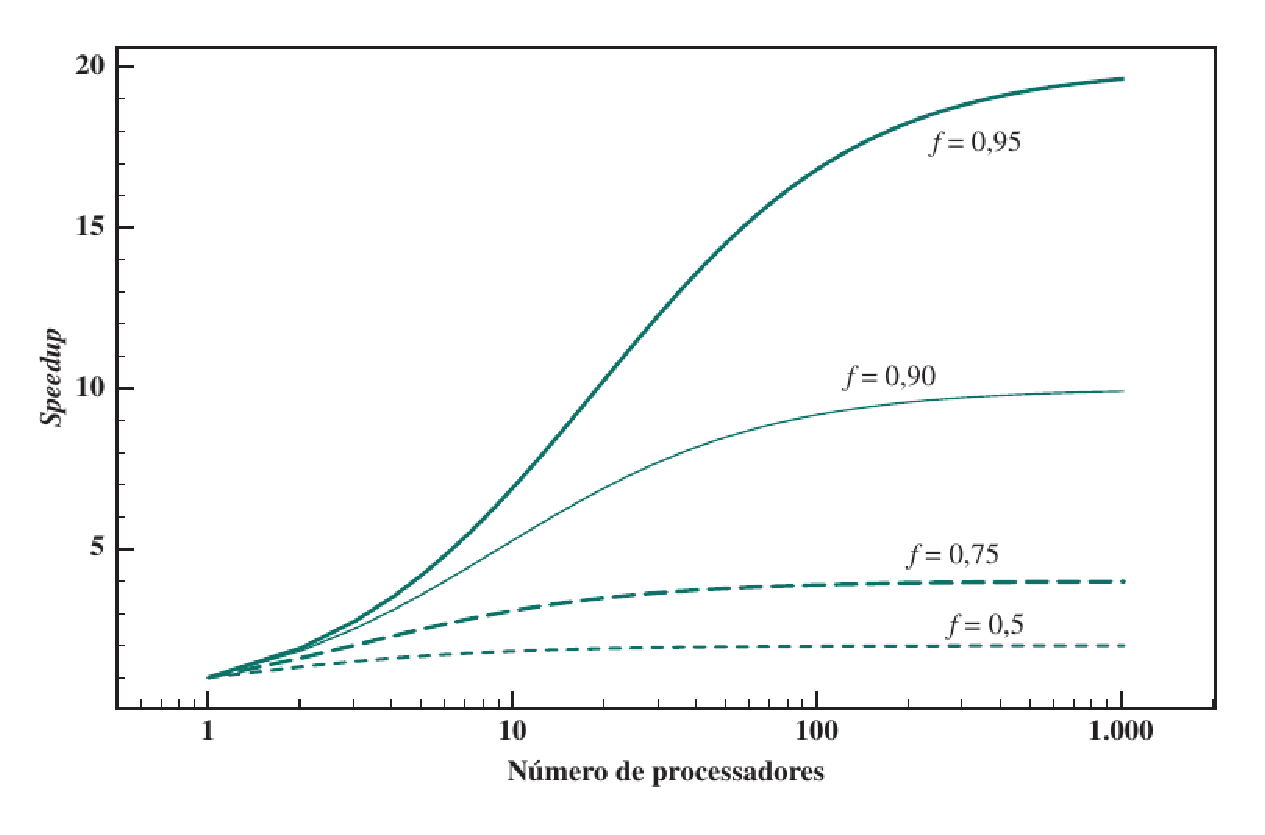
\includegraphics[width=0.7\textwidth]{figs/amdahl2}
			\end{center}
	\end{itemize}
\end{slide}


\begin{slide}{Lei de Amdahl generalizada}
\begin{itemize}
   \item Caracteriza o \textit{speedup} de um programa otimizado por qualquer processo:
   \begin{align*}
	   \text{Speedup} &= \frac{\text{tempo de execução antes da melhoria}}{\text{tempo de execução após a melhoria}}\\
              &= \frac{\text{desempenho após a melhoria}}{\text{desempenho antes da melhoria}}\\
              &= \frac{1}{(1-f)+\frac{f}{SU_f}}\\
   \end{align*}
   onde $SU_f$ corresponde ao \textit{speedup} da fração otimizada.
\end{itemize}
\end{slide}

\begin{slide}{Lei de Little}
	\begin{itemize}
		\item Considere um sistema (fila) em que itens chegam a uma taxa média $\lambda$ (itens por unidade de tempo)
		\item Cada item permanece no sistema, em média, por $W$ unidades de tempo
		\item A quantidade de itens no sistema ($L$) em determinado tempo é (em média):
			\begin{equation*}
				L = \lambda W
			\end{equation*}
		\item O sistema (fila) neste caso representa qualquer serviço prestado, enquanto os itens são solicitações ou tarefas demandadas:
			\begin{itemize}
				\item Atendimento de clientes no balcão da padaria
				\item Tempo para entrega de notas da prova
				\item Execução de \emph{threads} em sistemas multicore com acesso à memória compartilhado
				\item Distribuição de pacotes em transmissão de dados via rede
			\end{itemize}
	\end{itemize}
\end{slide}

\section[slide=true]{Medidas básicas de avaliação de desempenho de computadores}
\begin{slide}{Alguns fatores importantes}
\begin{itemize}
	\item Avaliação de um sistema compreende:
		\begin{itemize}
			\item Custo
			\item Tamanho
			\item Segurança
			\item Confiabilidade
			\item Consumo de energia
			\item Desempenho (velocidade de processamento)
		\end{itemize}\pause
	\item Fatores que influenciam o desempenho (em uma dada aplicação):
		\begin{itemize}
			\item Velocidade do processador
			\item Conjunto de instruções da máquina
			\item Escolha da linguagem de implementação
			\item Eficiência do compilador
			\item Habilidade do programador
		\end{itemize}
\end{itemize}
\end{slide}

\begin{slide}{Velocidade de \emph{clock}}
	\twocolumn{
		\begin{itemize}
			\item O \emph{clock} define o ritmo do processador: busca, decodificação, e execução de instruções\pause
			\item O valor do \emph{clock} não é arbitrário: deve observar os atrasos de propagação dos sinais nos circuitos digitais\pause
			\item Por que o \emph{clock} não é tudo em termos de desempenho?
				\begin{itemize}
					\item Diferentes instruções exigem um número diferente de ciclos para ser executadas
					\item Máquinas com \textit{pipeline}: várias instruções em execução simultaneamente
				\end{itemize}
		\end{itemize}
		}{
		\begin{center}
			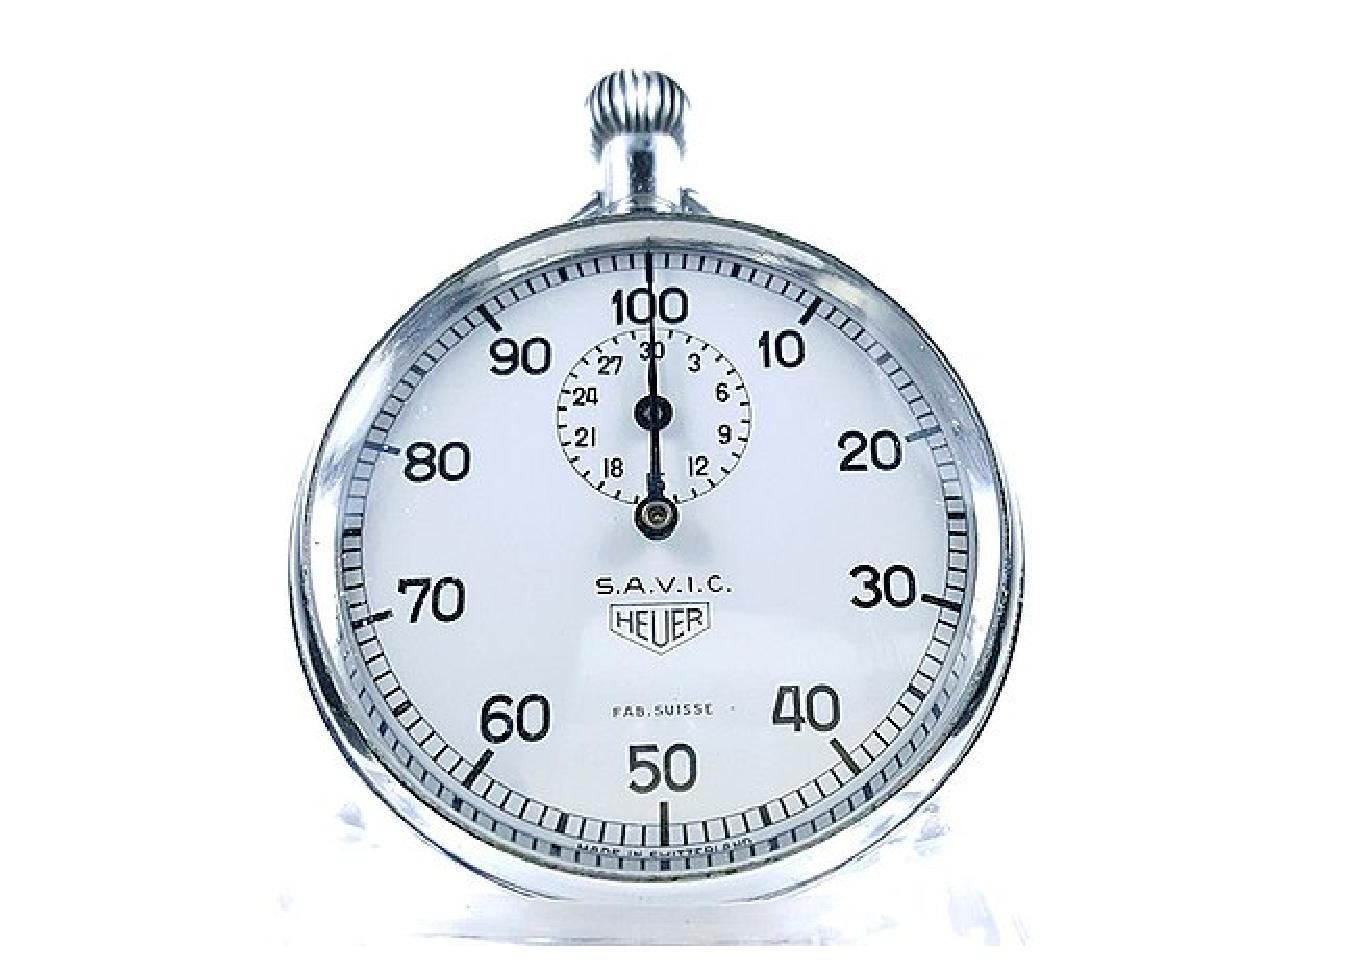
\includegraphics[width=0.9\textwidth]{figs/stopwatch}
			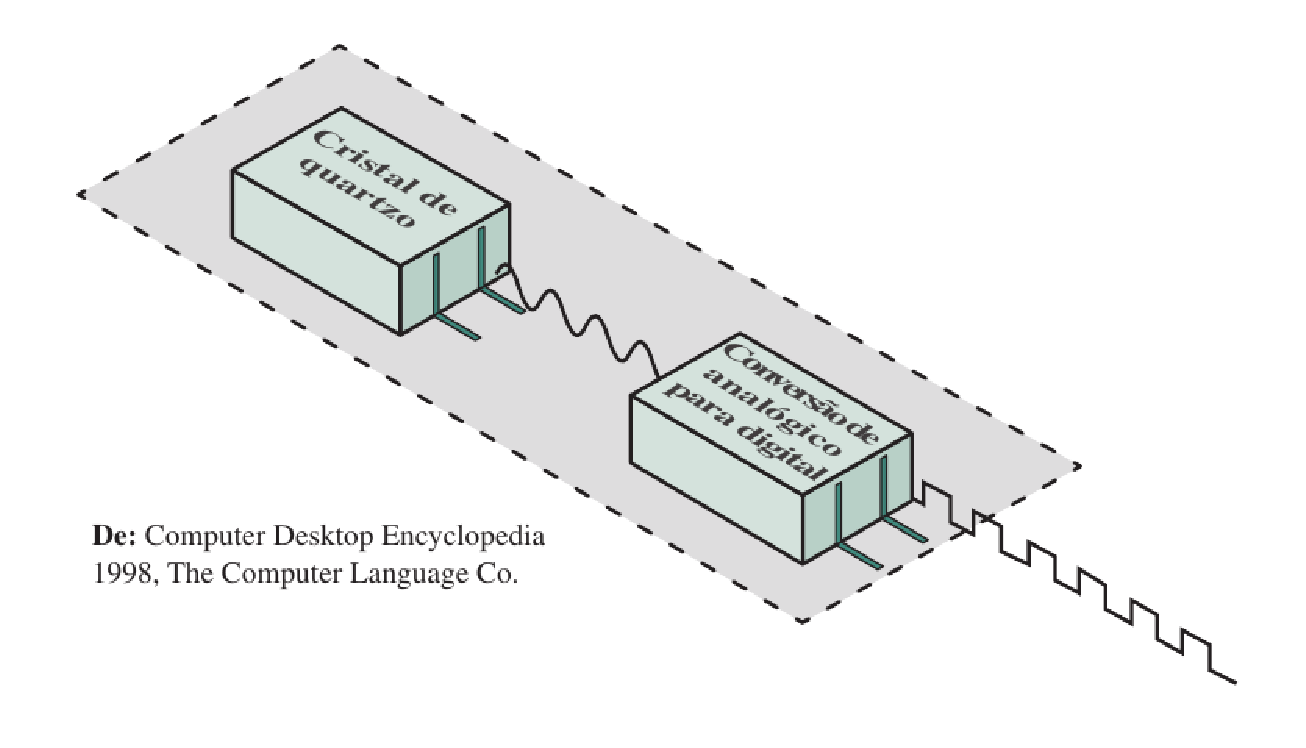
\includegraphics[width=0.9\textwidth]{figs/clock}
		\end{center}
		}
\end{slide}

\begin{slide}{Taxa de execução de instruções}
\begin{itemize}
   \item Ciclos por instrução médio ($CPI$):
   \begin{equation}
       CPI = \frac{\sum_{i = 1}^{n} CPI_i\times I_i}{I_c}
   \end{equation}
   \begin{itemize}
      \item $i$ representa o tipo de instrução; 
      \item $I_i$ denota o número de instruções do tipo $i$; 
      \item $CPI_i$ corresponde ao número de ciclos necessários para executar uma instrução do tipo $i$; 
      \item $I_c$ é o número total de instruções de um determinado programa; 
      \item $n$ é o número total de tipos de instruções.
   \end{itemize}
\end{itemize}
\end{slide}

\begin{slide}{Taxa de execução de instruções}
\begin{itemize}
	\item Tempo de execução ($T$):
		\begin{equation*}
			T = I_c \times CPI\times \tau
		\end{equation*}
		onde $\tau = 1/f$ é o tempo de um período do \emph{clock} ($f$: frequência do \emph{clock}).
	\item Refinamento:
		\begin{equation*}
			T = I_c \times \left [ p + \left ( m\times k \right )\right ]\times \tau
		\end{equation*}
		onde :
		\begin{itemize}
			\item $p$ é o número de ciclos para decodificar e executar um \emph{instrução média} 
			\item $m$ é o número de referências à memória necessário 
			\item $k$ é a razão entre o tempo de ciclo da memória e o tempo de ciclo do processador 
		\end{itemize}
\end{itemize}
\end{slide}

\begin{slide}{Taxa de execução de instruções}
	\begin{itemize}
		\item {CPI e tipos de instruções}
			\begin{center}
				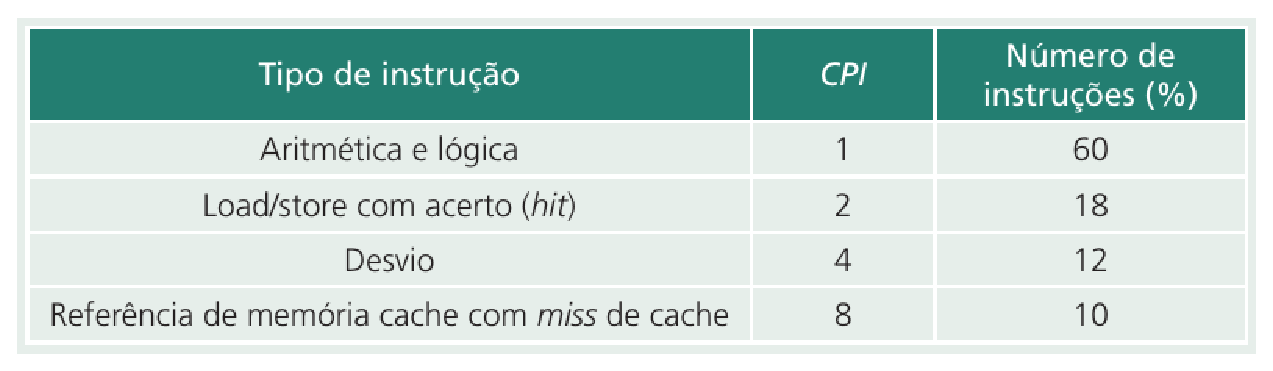
\includegraphics[width=0.8\textwidth]{figs/cpi} 
			\end{center} 
	\end{itemize}
\end{slide}

\begin{slide}{Taxa de execução de instruções}
\begin{itemize}
   \item Milhões de instruções por segundo -- MIPS:
	   \begin{equation*}
		   MIPS = \frac{I_c}{T\times 10^6} = \frac{f}{CPI\times 10^6}
	   \end{equation*}
   \item Milhões de operações de ponto flutuante por segundo -- MFLOPS
	   \begin{equation*}
		   MFLOPS = \frac{\text{número de operações de ponto flutuante}}{T\times 10^6}
	   \end{equation*}
\end{itemize} 
\end{slide}

\section[slide=true]{Cálculo de médias}
\begin{slide}{Definições}
	\begin{itemize}
		\item As médias servem para caracterizar um atributo que pode variar dependendo das condições de execução
		\item Média aritmética:
			\begin{equation*}
				m_a = \sum_{i=1}^n x_i
			\end{equation*}
		\item Média geométrica:
			\begin{equation*}
				m_g = \left (\prod_{i=1}^n  x_i \right )^{1/n} = \exp \left \{ \frac{1}{n}\sum_{i=1}^n \ln \left ( x_i \right ) \right \}
			\end{equation*}
		\item Média harmônica:
			\begin{equation*}
				m_h = \frac{n}{ \sum\limits_{i=1}^n \frac{1}{x_i}  }
			\end{equation*}
	\end{itemize}
\end{slide}

\section[slide=true]{Benchmarks e SPEC}
\begin{slide}{Benchmarks: motivação e princípios}
Mesmo as taxas MIPS e MFLOPS podem ser inadequadas:\\
\begin{itemize}
 \item Ex.: Executar A=B+C\\
\begin{itemize}
   \item Máquina CISC (1 MIPS)\\
   \texttt{add mem(B), mem(C), mem(A)}
   
   \item Máquina RISC (4 MIPS)\\
   \texttt{load mem(B), reg(1);\\
       load mem(C), reg(2);\\
       add  reg(1), reg(2), reg(3);\\
       store reg(3), mem(A)}
\end{itemize}
   \item Benchmark são: 
   \begin{itemize}
      \item Programas elaborados para testar o desempenho em determinado contexto;
      \item Escritos em linguagem de alto nível;
      \item Portáveis.
\end{itemize}
\end{itemize}
\end{slide}

\begin{slide}{Benchmarks SPEC}
\begin{itemize}
	\item SPEC: \textit{Standard Performance Evaluation Corporation}
	\item SPEC CPU2006: aplicações intensivas para o processador (não E/S)
		\begin{itemize}
			\item Desempenho em aplicações que gastam a maior parte do tempo na realização de cálculos
			\item 17 programas para avaliação de processamento de ponto flutuante em C, C++, Fortran.
			\item 12 programas para avaliação de processamento de inteiros em C, C++.
			\item São mais de 3 milhões de linhas de código.
		\end{itemize}
\end{itemize}
\end{slide}

\begin{slide}{Outras suítes SPEC}
\begin{itemize}
	\item SPECviewperf: avaliação de desempenho em gráficos 3D em aplicações profissionais
	\item SPECwpc: avaliação de aspectos-chave no desempenho de estações de trabalho
	\item SPECjvm2008: desempenho de hardware e software da plataforma cliente JVM
      \item SPECjbb2013: desempenho de aplicações de comércio eletrônico baseadas em Java (lado servidor)
      \item SPECcfs2008: avaliação da velocidade e capacidade no gerenciamento de requisições de servidores de arquivos
      \item SPECvirt\_sc2014: avaliação de desempenho de servidores de virtualização
\end{itemize}
\end{slide}

\begin{slide}{Fluxo de avaliação SPEC}
	\begin{center}
		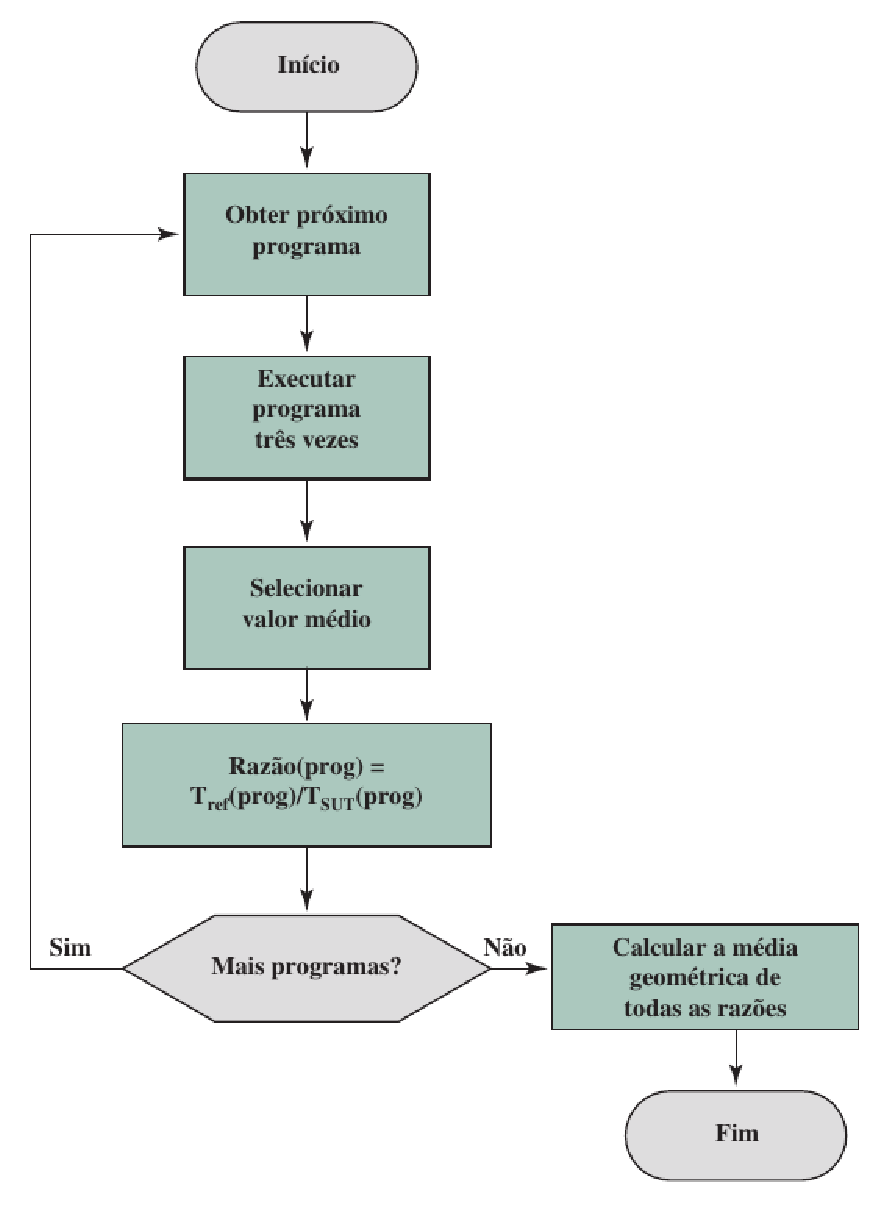
\includegraphics[height = 0.8\textheight]{figs/fluxo-spec}
	\end{center}
\end{slide}
\end{document}
